\section{Explication des projets}

% Un titre de section aussi long est \textbf{fortement déconseillé} mais j'ai configuré le header pour qu'il le gère.

\subsection{Projet Gaia}

\subsubsection{Contexte}
~\\
Le projet GAIA vise à simplifier l'utilisation des rapports de durabilité des entreprises grâce à une plateforme centralisée et à faciliter la recherche en réduisant les efforts manuels. 
Il cherche également à créer une référence fiable pour les informations liées au climat.

Ce projet a été lancé par la Deutsche Bundesbank en réponse à la prise de conscience croissante de l'importance de la finance durable.
En effet, des risques financiers en découlent, et il faut donc en avoir conscience et savoir les gérer.

La motivation derrière le projet GAIA est de fournir aux investisseurs et aux décideurs des informations fiables et cohérentes sur la durabilité des investissements. 
Il s'agit de donner aux investisseurs les moyens de prendre des décisions d'investissement plus éclairées et de mieux comprendre les risques et les opportunités associés aux investissements durables.

La Bundesbank a également pour objectif de promouvoir la stabilité financière en intégrant les risques liés au changement climatique dans ses analyses et en encourageant les investisseurs à intégrer ces risques dans leur propre prise de décision.
\\
L'équipe du projet est composée de membres de la Bundesbank bien sûr, mais se fait surtout en collaboration avec d'autres banques internationales (Banque d'Espagne, Banque Centrale Européenne, etc...).

Concrètement, le projet consiste tout d'abord à récupérer les rapports de durabilité des entreprises, disponibles publiquement en ligne.
Ensuite, le texte et les tableaux / graphiques sont extraits, et les données d'empreinte carbone des entreprises (Scope 1, 2, 3) sont extraites à l'aide de Natural Language Processing (NLP).

\begin{figure}[H]
    \centering
    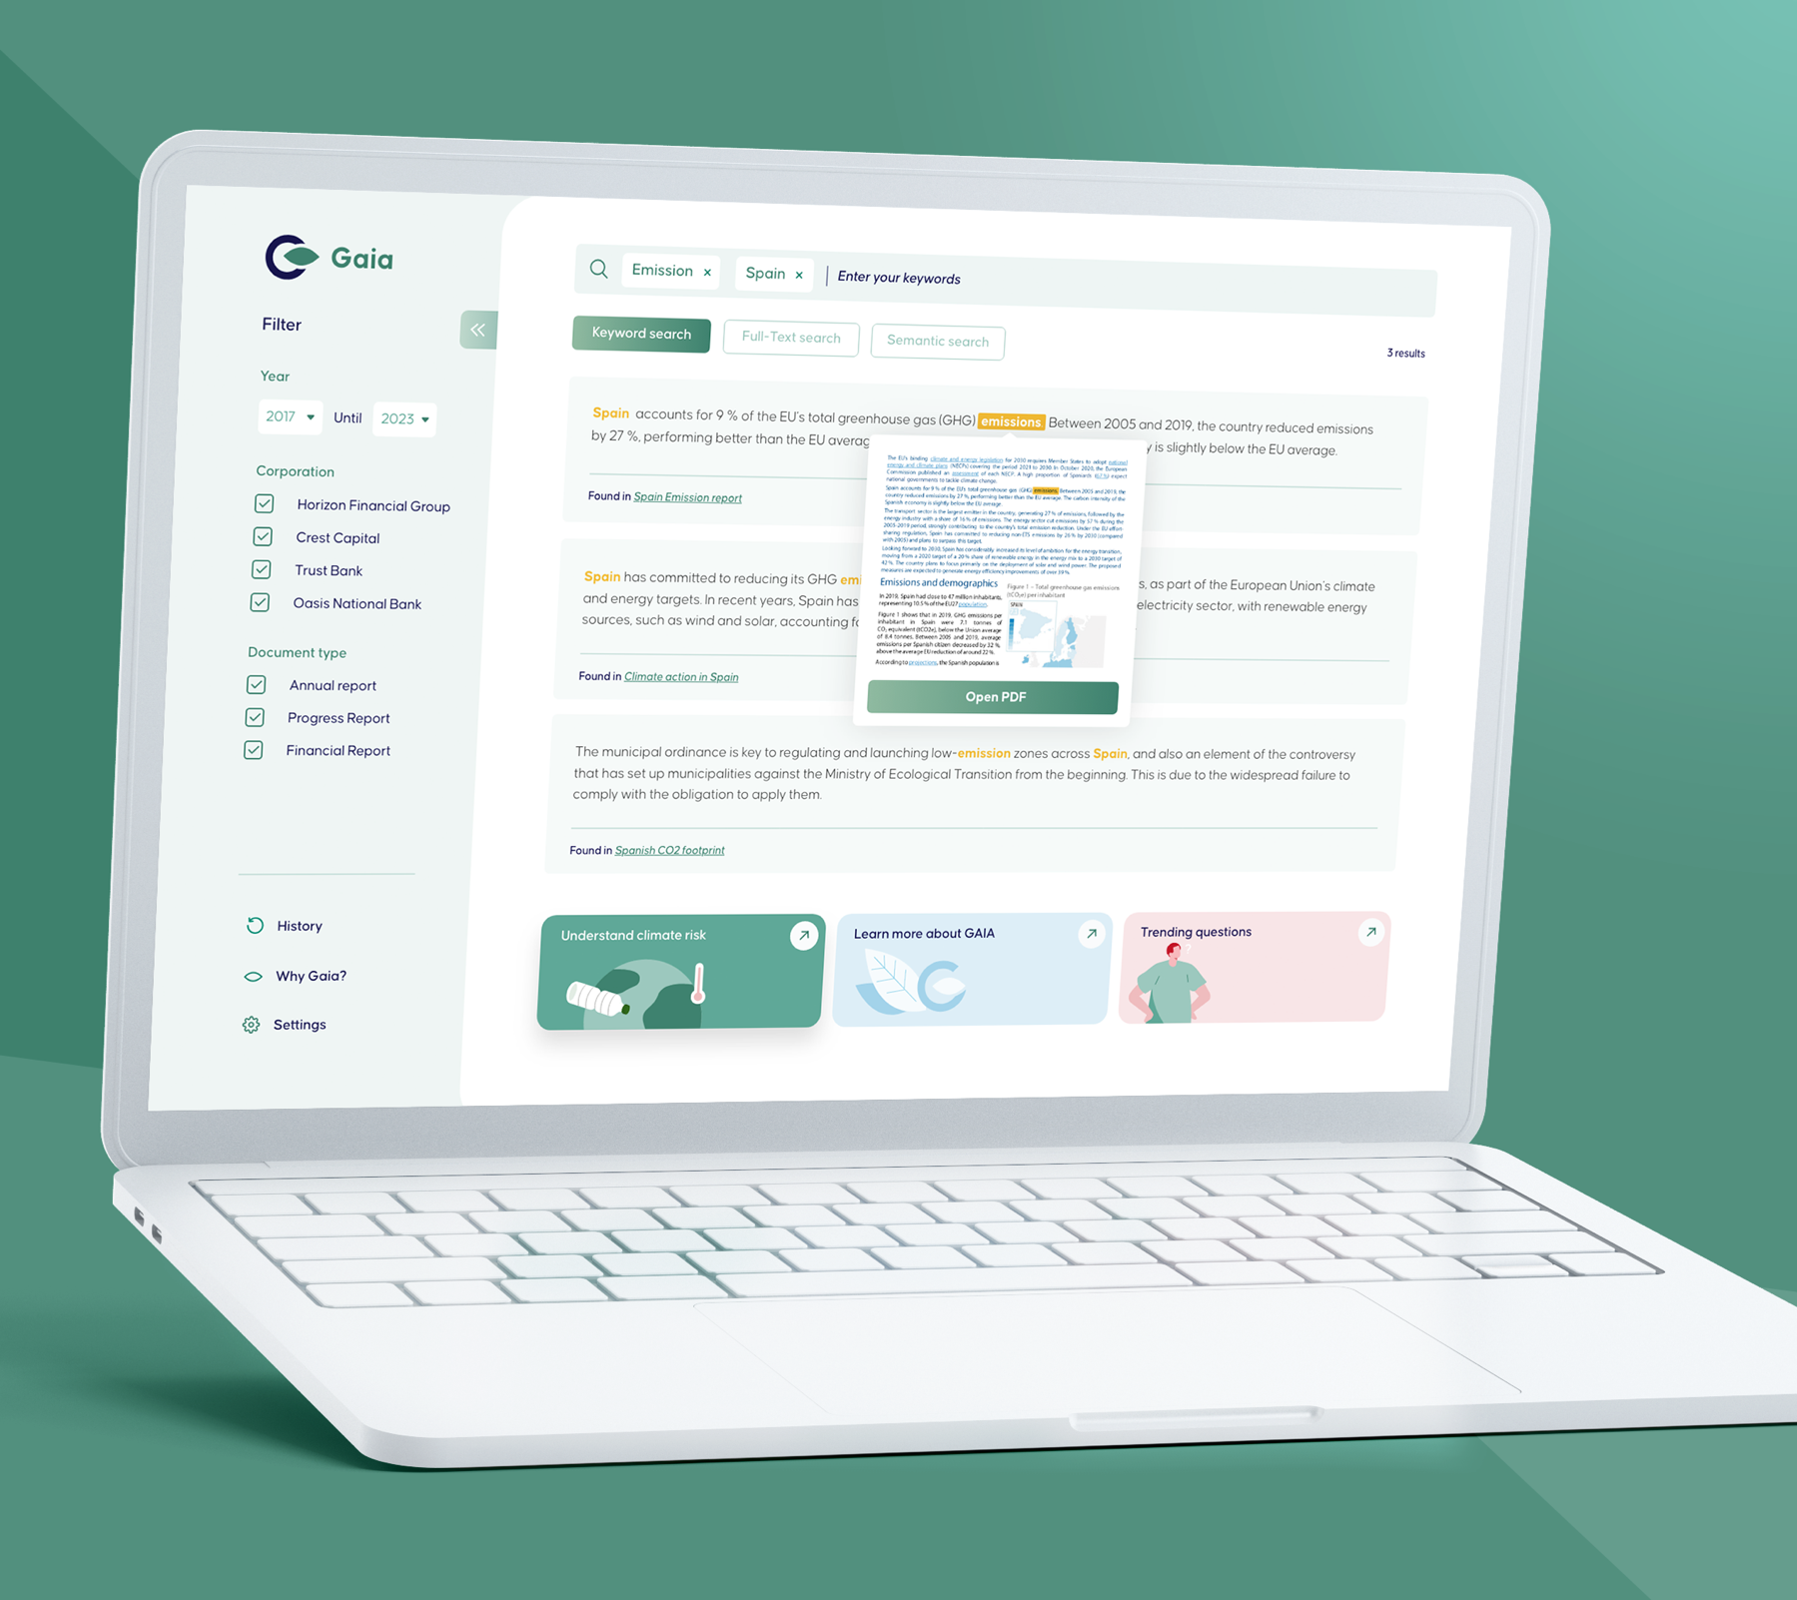
\includegraphics[width=12cm]{GAIA.png}
    \caption{Mock-up de la plateforme Gaia}
\end{figure}

\subsubsection{Antécédents}
~\\
Mises à part les spécifications et objectifs de la plateforme qui étaient dejà clairs, rien n'avait été concrètement commencé avant mon arrivée.
\subsubsection{Objectif visé}

L'objectif est de présenter une preuve de concept du projet.
Mon principal objectif était donc de développer un crawler qui parcourerait les résultats de recherche Google pour les rapports de durabilité des entreprises majeures dans le monde.
Les PDFs trouvés doivent ensuite être téléchargés. 
Parallèlement, les PDFs/liens trouvés doivent être classés, selon s'ils sont justes ou faux pour une requête donnée.
Une fois que cela serait fait, je devrais présenter mes résultats à l'équipe du projet.

\pagebreak
\subsection{Projet ESCB Exchange}

\subsubsection{Contexte}
~\\
ESCB signifie Eurosystem/European System of Central Banks. Cela se réfère au système européen de banques centrales. 
L'Eurosystem est composé de la Banque centrale européenne (BCE) et des banques centrales nationales des pays de la zone euro. 

L'ESCB Exchange est un forum permettant aux banques centrales de collaborer autour de données climatiques communes. 
Ce forum favorise l'échange de connaissances, de code et d'applications pour améliorer la valeur analytique des données climatiques utilisées. 
Chaque banque centrale désigne jusqu'à 2 experts en données climatiques pour participer au forum. 
Les rencontres du forum ont lieu chaque mois, et des groupes volontaires et agiles pilotent les sujets d'intérêt commun. 
L'initiative encourage l'échange sur le nettoyage des données, le partage de code et les leçons apprises concernant les données climatiques granulaires (des entreprises).

L'un des sujets abordés lors des forums est notamment le rapprochement de données sur les émissions carbones, censées être identiques mais provenant de différentes sources.
En effet, les banques collectent ces données et les utilisent pour des recherches. Il est donc primordial de choisir la meilleure source de données climatiques.
Ma mission portait exactement là-dessus.

\subsubsection{Antécédents}
~\\
Concernant le rapprochement de données provenant de différentes sources, un code d'analyses de données en R ainsi qu'une présentation présentant la comparaison avaient déjà été faits.
La comparaison concernait les sources ISS et Carbon 4 Finance, tous deux fournisseurs de données. 

\subsubsection{Objectif visé}
~\\
Ma mission consistait en la même analyse que celle faite précédemment, sauf qu'au lieu de faire une analyse bilatérale, je devais en faire une trilatérale en ajoutant aux sources précédentes celle de TRUCOST.
Le Powerpoint associé devait également être fait en aval.

\begin{figure}[H]
    \centering
    
\includegraphics[width=12cm]{ESCB logos.png}
    \caption{Logos des sources de données à rapprocher}
\end{figure}

\pagebreak

\subsection{Projet CSDB}

\subsubsection{Contexte}
~\\
CSDB signifie "Central Securities Database". Il s'agit d'une base de données centrale des titres en Allemagne, utilisée pour la surveillance des marchés financiers, le suivi des transactions de titres et la facilitation des processus de règlement-livraison.
Au sein de la DSZ, les chercheurs utilisent cette base de données.
\\

Les datasets sont sous la forme de fichiers CSV et il y en a 1 pour chaque mois de chaque année depuis 2009.
Tous les mois environ, une nouvelle version d'un ou plusieurs de ces datasets peut parfois être générée, avec des nouvelles colonnes, nouvelles valeurs, etc...
Autrement dit, une nouvelle version du dataset de 2022-04 (différente de l'original) peut être créée en Avril 2023.

Pour chaque dataset, 4 variantes doivent être générées : En effet, des normes existent, et chaque groupe de chercheurs possède des droits de lecture différents sur les colonnes du dataset.
Par conséquent, chaque variante possède le même contenu dans ses colonnes, mais les colonnes présentes sont différentes.
Et cela doit être fait dès qu'une nouvelle version d'un dataset existe.
Or, chaque dataset fait plusieurs Go, et actuellement, cette génération des 4 variantes ainsi que la comparaison de chaque nouveau dataset avec sa version originale prend 1 semaine. 
\\

Quand la procédure doit être répétée tous les mois, cette solution n'est pas viable telle quelle et doit être optimisée.

\subsubsection{Antécédents}
~\\
La situation à mon arrivée était la suivante :

Les nouvelles et les anciennes versions du "même" ensemble de données (par exemple les données 2009-04) étaient comparées après la génération des 4 ensembles de données.
Cela engendre beaucoup d'effort et de temps de calcul évitable.

Les fichiers csv ont été compressés afin de tenter une baisse du temps, ce qui a effectivement beaucoup accéléré le temps de lecture des csv. 
Cependant le temps de compression semblait fortement ralentir le processus. 

La comparaison des datasets comportait trop d'informations (moyenne, médiane de chaque colonne des datasets, et bien d'autres valeurs statistiques), ce qui utilisait très certainement du temps supplémentaire inutile, quand seulement un très bref résultat était attendu.

\subsubsection{Objectif visé}
~\\
Afin de pouvoir générer les 4 versions de datasets uniquement sur les versions modifiées des jeux de données de la même période, la comparaison doit être réalisée en amont.
De plus, la comparaison doit être optimisée et n'indiquer à la fin que si les datasets sont identiques ou non, et sinon montrer les différences.

\pagebreak
\subsection{Projet NFiG}

\subsubsection{Contexte}
~\\
NFiG signifie "pour usage interne seulement" (Nur für internen Gebrauch) et concerne les données des chercheurs du département. 
Ces derniers utilisent Stata, un logiciel de statistiques pour générer des graphiques ou effectuer différentes analyses.
Lorsque ces graphiques doivent être publiés, ils doivent être adaptés de manière à ne plus être confidentiels.

Par conséquent, chaque graphique doit être retrouvé dans le code qui l'a généré, ce qui implique de connaître le fichier stata et la ligne à laquelle l'output est généré.

Le but est donc de retrouver automatiquement où est créé chaque graphe dans le code, ou de manière plus générale, de faciliter leur "traçage".
Or, les exportations peuvent être générées par des boucles, ce qui rend la recherche des noms de fichiers difficile.

\subsubsection{Antécédents}
~\\
Un code python avait déjà été écrit pour tenter d'automatiser cette recherche, mais n'a pas vraiment réussi.
Des rapports Excel on été faits à la main afin de recenser quel graphique ou autre fichier output a été généré dans quel fichier de code / fichier log et à quelle ligne. 

\subsubsection{Objectif visé}
~\\ La tâche qui m'a été donnée

\pagebreak

\subsection{Projet de recherche NLP}

\subsubsection{Contexte}
~\\
\subsubsection{Antécédents}
~\\
\subsubsection{Objectif visé}
